% Options for packages loaded elsewhere
% Options for packages loaded elsewhere
\PassOptionsToPackage{unicode}{hyperref}
\PassOptionsToPackage{hyphens}{url}
%
\documentclass[
  ignorenonframetext,
  ngerman,
]{beamer}
\newif\ifbibliography
\usepackage{pgfpages}
\setbeamertemplate{caption}[numbered]
\setbeamertemplate{caption label separator}{: }
\setbeamercolor{caption name}{fg=normal text.fg}
\beamertemplatenavigationsymbolsempty
% remove section numbering
\setbeamertemplate{part page}{
  \centering
  \begin{beamercolorbox}[sep=16pt,center]{part title}
    \usebeamerfont{part title}\insertpart\par
  \end{beamercolorbox}
}
\setbeamertemplate{section page}{
  \centering
  \begin{beamercolorbox}[sep=12pt,center]{section title}
    \usebeamerfont{section title}\insertsection\par
  \end{beamercolorbox}
}
\setbeamertemplate{subsection page}{
  \centering
  \begin{beamercolorbox}[sep=8pt,center]{subsection title}
    \usebeamerfont{subsection title}\insertsubsection\par
  \end{beamercolorbox}
}
% Prevent slide breaks in the middle of a paragraph
\widowpenalties 1 10000
\raggedbottom
\AtBeginPart{
  \frame{\partpage}
}
\AtBeginSection{
  \ifbibliography
  \else
    \frame{\sectionpage}
  \fi
}
\AtBeginSubsection{
  \frame{\subsectionpage}
}
\usepackage{iftex}
\ifPDFTeX
  \usepackage[T1]{fontenc}
  \usepackage[utf8]{inputenc}
  \usepackage{textcomp} % provide euro and other symbols
\else % if luatex or xetex
  \usepackage{unicode-math} % this also loads fontspec
  \defaultfontfeatures{Scale=MatchLowercase}
  \defaultfontfeatures[\rmfamily]{Ligatures=TeX,Scale=1}
\fi
\usepackage{lmodern}

\usetheme[]{Madrid}
\usecolortheme[]{default}
\ifPDFTeX\else
  % xetex/luatex font selection
\fi
% Use upquote if available, for straight quotes in verbatim environments
\IfFileExists{upquote.sty}{\usepackage{upquote}}{}
\IfFileExists{microtype.sty}{% use microtype if available
  \usepackage[]{microtype}
  \UseMicrotypeSet[protrusion]{basicmath} % disable protrusion for tt fonts
}{}
\makeatletter
\@ifundefined{KOMAClassName}{% if non-KOMA class
  \IfFileExists{parskip.sty}{%
    \usepackage{parskip}
  }{% else
    \setlength{\parindent}{0pt}
    \setlength{\parskip}{6pt plus 2pt minus 1pt}}
}{% if KOMA class
  \KOMAoptions{parskip=half}}
\makeatother


\usepackage{longtable,booktabs,array}
\usepackage{calc} % for calculating minipage widths
\usepackage{caption}
% Make caption package work with longtable
\makeatletter
\def\fnum@table{\tablename~\thetable}
\makeatother
\usepackage{graphicx}
\makeatletter
\newsavebox\pandoc@box
\newcommand*\pandocbounded[1]{% scales image to fit in text height/width
  \sbox\pandoc@box{#1}%
  \Gscale@div\@tempa{\textheight}{\dimexpr\ht\pandoc@box+\dp\pandoc@box\relax}%
  \Gscale@div\@tempb{\linewidth}{\wd\pandoc@box}%
  \ifdim\@tempb\p@<\@tempa\p@\let\@tempa\@tempb\fi% select the smaller of both
  \ifdim\@tempa\p@<\p@\scalebox{\@tempa}{\usebox\pandoc@box}%
  \else\usebox{\pandoc@box}%
  \fi%
}
% Set default figure placement to htbp
\def\fps@figure{htbp}
\makeatother



\ifLuaTeX
\usepackage[bidi=basic]{babel}
\else
\usepackage[bidi=default]{babel}
\fi
% get rid of language-specific shorthands (see #6817):
\let\LanguageShortHands\languageshorthands
\def\languageshorthands#1{}
\ifLuaTeX
  \usepackage[german]{selnolig} % disable illegal ligatures
\fi


\setlength{\emergencystretch}{3em} % prevent overfull lines

\providecommand{\tightlist}{%
  \setlength{\itemsep}{0pt}\setlength{\parskip}{0pt}}



 


\makeatletter
\@ifpackageloaded{caption}{}{\usepackage{caption}}
\AtBeginDocument{%
\ifdefined\contentsname
  \renewcommand*\contentsname{Inhaltsverzeichnis}
\else
  \newcommand\contentsname{Inhaltsverzeichnis}
\fi
\ifdefined\listfigurename
  \renewcommand*\listfigurename{Abbildungsverzeichnis}
\else
  \newcommand\listfigurename{Abbildungsverzeichnis}
\fi
\ifdefined\listtablename
  \renewcommand*\listtablename{Tabellenverzeichnis}
\else
  \newcommand\listtablename{Tabellenverzeichnis}
\fi
\ifdefined\figurename
  \renewcommand*\figurename{Abbildung}
\else
  \newcommand\figurename{Abbildung}
\fi
\ifdefined\tablename
  \renewcommand*\tablename{Tabelle}
\else
  \newcommand\tablename{Tabelle}
\fi
}
\@ifpackageloaded{float}{}{\usepackage{float}}
\floatstyle{ruled}
\@ifundefined{c@chapter}{\newfloat{codelisting}{h}{lop}}{\newfloat{codelisting}{h}{lop}[chapter]}
\floatname{codelisting}{Listing}
\newcommand*\listoflistings{\listof{codelisting}{Listingverzeichnis}}
\makeatother
\makeatletter
\makeatother
\makeatletter
\@ifpackageloaded{caption}{}{\usepackage{caption}}
\@ifpackageloaded{subcaption}{}{\usepackage{subcaption}}
\makeatother

\usepackage{bookmark}
\IfFileExists{xurl.sty}{\usepackage{xurl}}{} % add URL line breaks if available
\urlstyle{same}
\hypersetup{
  pdftitle={Was macht ein Teilchenphysiker?},
  pdfauthor={Gianluca · Doktorand · Theoretische Teilchenphysik},
  pdflang={de},
  hidelinks,
  pdfcreator={LaTeX via pandoc}}


\title{Was macht ein Teilchenphysiker?}
\subtitle{Lattice QCD -- Quarks auf dem Gitter}
\author{Gianluca · Doktorand · Theoretische Teilchenphysik}
\date{2026-04-17}

\begin{document}
\frame{\titlepage}


\begin{frame}{Warum Teilchenphysik?}
\phantomsection\label{warum-teilchenphysik}
\note{Kurz vorstellen: Name, Promotion, warum ich Physik mache.}

\begin{columns}[T]
\begin{column}{0.55\linewidth}
\begin{itemize}
\tightlist
\item
  Woraus besteht die Welt wirklich?
\item
  Warum haben Teilchen Masse?
\item
  Was hält Protonen \& Neutronen zusammen?
\item
  Lassen sich mathematische Formeln zur Beschreibung der Natur finden?
\end{itemize}
\end{column}

\begin{column}{0.45\linewidth}
\begin{figure}[H]

{\centering 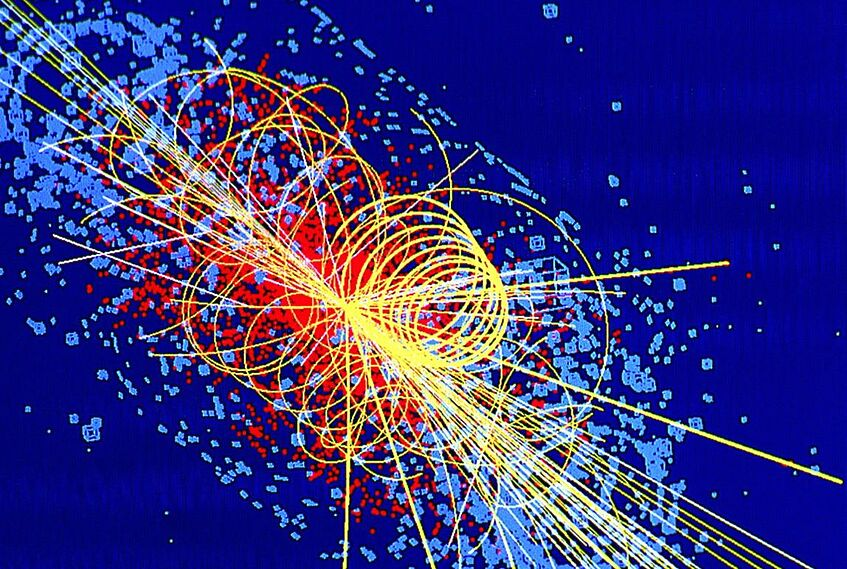
\includegraphics[width=1\linewidth,height=\textheight,keepaspectratio]{particlephysics.jpg}

}

\caption{https://particle.univie.ac.at/}

\end{figure}%
\end{column}
\end{columns}

\note{Alltagsbezug herstellen, Neugier wecken.}
\end{frame}

\begin{frame}{Das Standardmodell (Überblick)}
\phantomsection\label{das-standardmodell-uxfcberblick}
\begin{figure}[H]

{\centering 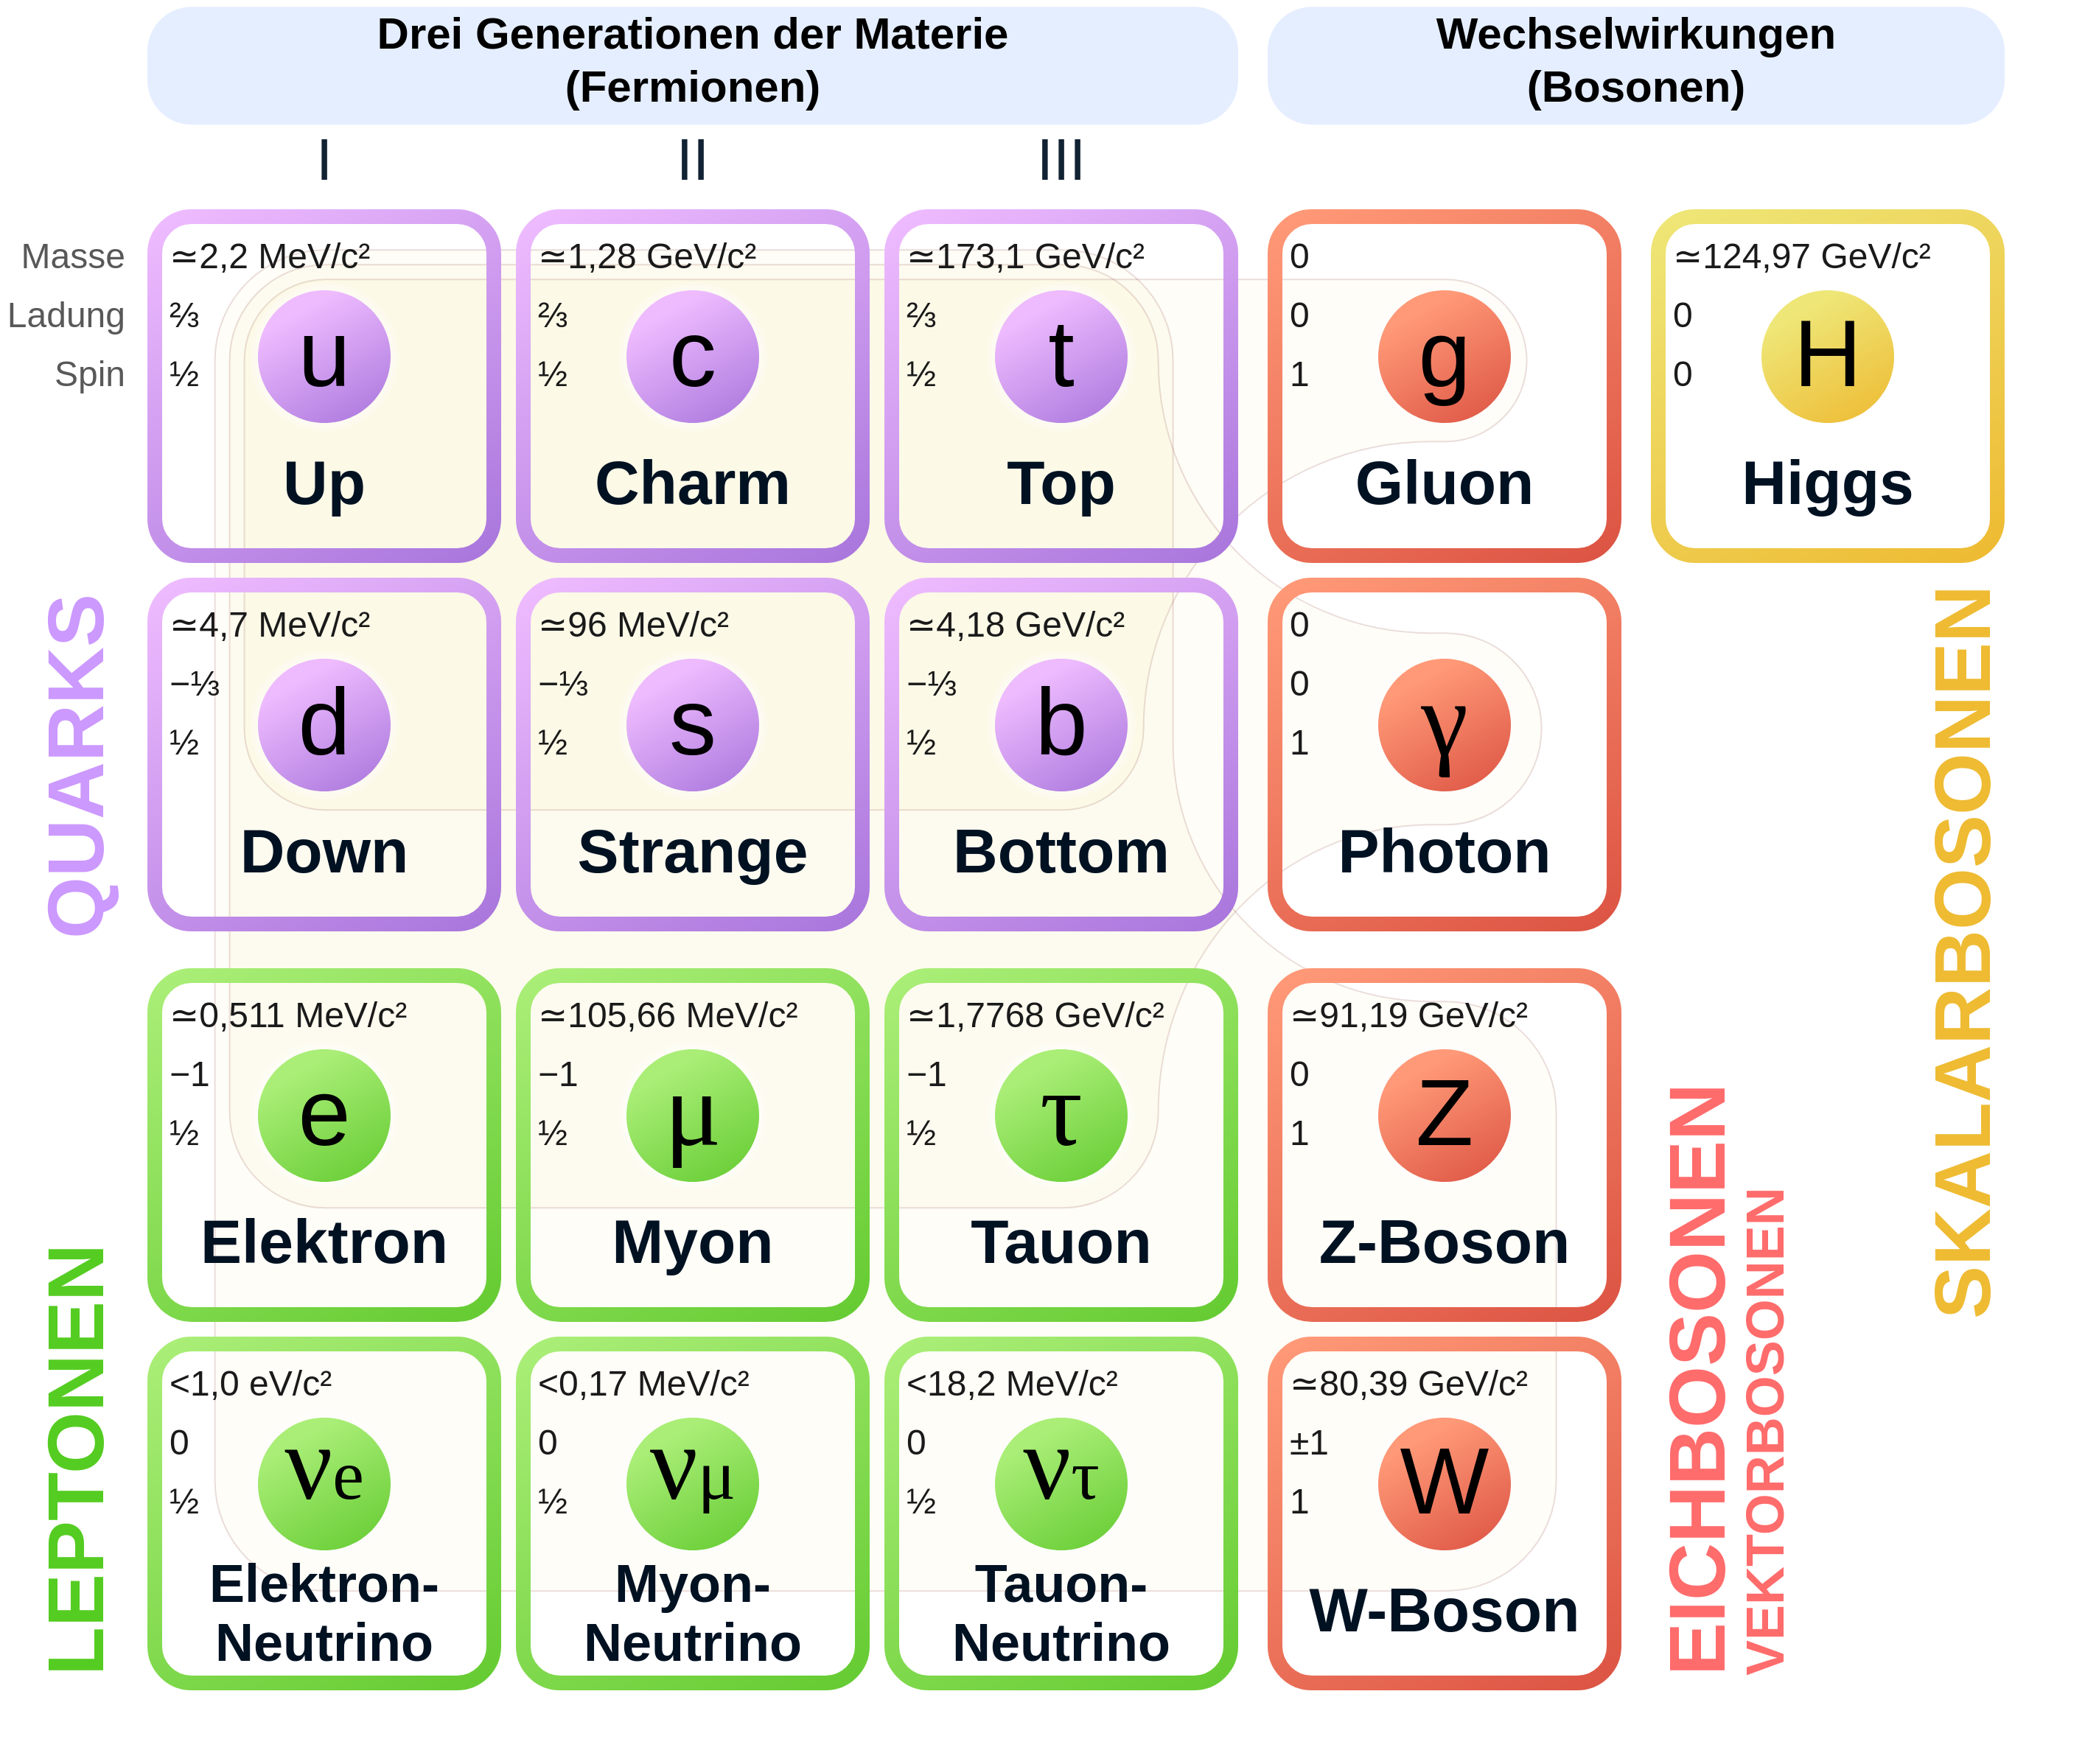
\includegraphics[width=0.63\linewidth,height=\textheight,keepaspectratio]{standardmodel.png}

}

\caption{Von MissMJ \& Cush / abgeleitetes Werk: Polluks - Standard
Model of Elementary Particles.svg, Gemeinfrei,
https://commons.wikimedia.org/w/index.php?curid=11307906}

\end{figure}%

\note{Betonung: Alles, was wir kennen. Fokus gleich auf Quarks \&
Gluonen lenken → QCD.}
\end{frame}

\begin{frame}{Die starke Wechselwirkung}
\phantomsection\label{die-starke-wechselwirkung}
\begin{columns}[T]
\begin{column}{0.45\linewidth}
\begin{itemize}
\tightlist
\item
  Beschrieben durch: \textbf{QCD} (Quantenchromodynamik)
\item
  Quarks tragen \emph{Farbladung}
\item
  Vermittelt durch Gluonen
\item
  Verantwortlich für \textasciitilde99\% der Masse sichtbarer Materie
\end{itemize}
\end{column}

\begin{column}{0.45\linewidth}
\begin{figure}[H]

{\centering 
\includegraphics[width=1\linewidth,height=\textheight,keepaspectratio]{index_files/mediabag/Quark_structure_proton.pdf}

}

\caption{By Arpad Horvath - Own work, CC BY-SA 2.5,
https://commons.wikimedia.org/w/index.php?curid=637353}

\end{figure}%
\end{column}
\end{columns}

\note{Farbe als Analogie, keine echte Farbe.}
\end{frame}

\begin{frame}{Das Problem}
\phantomsection\label{das-problem}
QCD-Gleichungen sind bekannt \ldots{}

\textbf{\ldots{} aber extrem schwer zu lösen!}

\pause

Warum?
\end{frame}

\begin{frame}{Klassische Physik vs.~Quantenphysik}
\phantomsection\label{klassische-physik-vs.-quantenphysik}
\begin{itemize}
\tightlist
\item
  {\textbf{Klassische Physik:}} Natur wählt den Pfad mit minimaler
  \emph{Wirkung}
\end{itemize}

Die \emph{Wirkung} ist eine Zahl, die angibt, wie sehr sich das
Universum ``anstrengen muss'' um einen Pfad durchzuführen (Analogon:
Effizienz)

\note{Pfadintegral-Idee nach Feynman. Betonung: viele Pfade
interferieren, klassischer Pfad dominiert.}
\end{frame}

\begin{frame}{Klassische Physik vs.~Quantenphysik}
\phantomsection\label{klassische-physik-vs.-quantenphysik-1}
\begin{itemize}
\tightlist
\item
  {\textbf{Klassische Physik:}} Natur wählt den Pfad mit minimaler
  Wirkung
\item
  {\textbf{Quantenphysik:}} Alle Pfade tragen bei, aber kleine Wirkung →
  größere Bedeutung
\end{itemize}

\pause

Aufsummierung und Mittelung aller Pfade wird als \emph{Pfadintegral}
bezeichnet

\note{Pfadintegral-Idee nach Feynman. Betonung: viele Pfade
interferieren, klassischer Pfad dominiert.}
\end{frame}

\begin{frame}{Pfadintegral in der QED}
\phantomsection\label{pfadintegral-in-der-qed}
Beispiel: \textbf{Elektron--Elektron-Streuung} (Elektronen werden
aufeinander geschossen) Ziel: Berechne die Wahrscheinlichkeit, dass das
Elektron in einem bestimmten Winkel gestreut wird und vergleiche mit
Experiment
\end{frame}

\begin{frame}{Pfadintegral in der QED}
\phantomsection\label{pfadintegral-in-der-qed-1}
Beispiel: \textbf{Elektron--Elektron-Streuung} (Elektronen werden
aufeinander geschossen) Ziel: Berechne die Wahrscheinlichkeit, dass das
Elektron in einem bestimmten Winkel gestreut wird und vergleiche mit
Experiment

Ein Diagramm = ein Term im Pfadintegral (Feynman-Diagramme)
\end{frame}

\begin{frame}{Pfadintegral in der QED}
\phantomsection\label{pfadintegral-in-der-qed-2}
Beispiel: \textbf{Elektron--Elektron-Streuung}

\pause

\textbf{Speziell in der QED}: Je mehr Wechselwirkungen, desto
unwichtiger werden Pfade (ist nicht immer so)
\end{frame}

\begin{frame}{Pfadintegral in der QED}
\phantomsection\label{pfadintegral-in-der-qed-3}
Beispiel: \textbf{Elektron--Elektron-Streuung}

→ Um Observablen zu berechnen und mit Experimenten vergleichen zu können
braucht man nur eine \textbf{endliche} Anzahl an Diagrammen
\end{frame}

\begin{frame}{Wichtige Klarstellung}
\phantomsection\label{wichtige-klarstellung}
\begin{itemize}
\tightlist
\item
  Feynman-Diagramme sind \textbf{keine echten Teilchenbahnen}
\item
  Sie sind ein mathematischer Trick
\item
  Hilfreich, um das Pfadintegral übersichtlich zu berechnen
\item
  Bewart uns fürs erste davor, tiefer in die \emph{Quantenfeldtheorie}
  gehen zu müssen
\end{itemize}

\note{Nicht als Zeitablauf interpretieren!}
\end{frame}

\begin{frame}{Und jetzt: QCD}
\phantomsection\label{und-jetzt-qcd}
\begin{itemize}
\tightlist
\item
  Starke Kopplung: Komplizierte Diagramme werden \textbf{nicht}
  unwichtig
\item
  Unendlich viele wichtige Diagramme
\end{itemize}

\pause

\textbf{→ Keine andere Wahl mehr, als mit Feldern zu rechnen!}

\note{Perfekter Übergang zur Gitteridee.}
\end{frame}

\begin{frame}{Rechnen in der Quantenfeldtheorie (QFT)}
\phantomsection\label{rechnen-in-der-quantenfeldtheorie-qft}
\begin{itemize}
\tightlist
\item
  Teilchen sind Anregungen verschiedener Quantenfelder
\item
  Für Rechnungen muss die Raumzeit diskretisiert werden
\item
  Hochdimensionale Integrale (meist mindestens \(10^6\) Variablen)
\item
  Kann nicht analytisch berechnet werden → Wir müssen Computer
  verwenden!
\item
  QCD auf dem Computer: \emph{Lattice QCD}
\end{itemize}

\pause

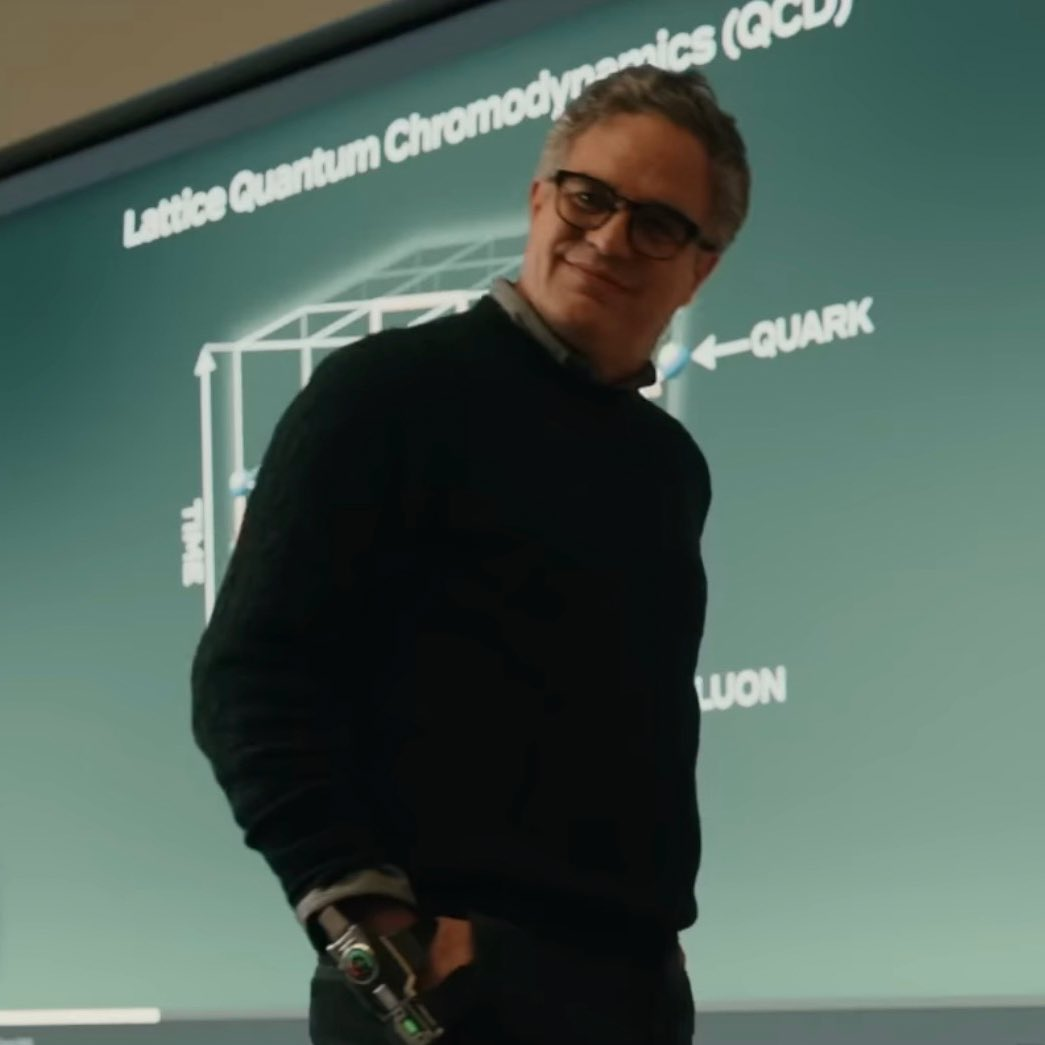
\includegraphics[width=0.25\linewidth,height=\textheight,keepaspectratio]{latticeqcd_spiderman.jpg}

\includegraphics[width=0.12\linewidth,height=\textheight,keepaspectratio]{shocked.png}
\end{frame}

\begin{frame}{Die Idee von Lattice QCD}
\phantomsection\label{die-idee-von-lattice-qcd}
\begin{columns}[T]
\begin{column}{0.5\linewidth}
\begin{itemize}
\tightlist
\item
  Beschränke das Universum auf ein \textbf{sehr kleines Volumen}
  (kleiner als ein Atom)
\item
  Raum und Zeit werden zum \emph{Gitter} (eng.: \emph{Lattice})
\item
  Quarks sitzen auf Gitterpunkten
\item
  Gluonen auf den Verbindungen
\item
  Genaue Größe des Gitters wird vor der Simulation festgelegt
\item
  Echte Physik bekommt man nur im Fall \emph{\(a \rightarrow 0\)}
\end{itemize}
\end{column}

\begin{column}{0.5\linewidth}
\end{column}
\end{columns}

\note{Vergleich mit Pixeln auf einem Bildschirm. Warum dieser trick
funktioniert ist etwas zu kompliziert für heute\ldots{}}
\end{frame}

\begin{frame}{Lattice QCD}
\phantomsection\label{lattice-qcd}
\textbf{Wie rechnet man jetzt auf dem Gitter?}

\begin{itemize}
\tightlist
\item
  Ähnlich zum Pfadintegral brauchen wir jetzt die wichtigen
  \textbf{Feldkonfigurationen}
\item
  Aber wie gesagt, gibt es in der QCD unendlich viele
\end{itemize}

\pause

\textbf{Brauchen wir denn wirklich alle?}
\end{frame}

\begin{frame}{Lattice QCD}
\phantomsection\label{lattice-qcd-1}
\begin{itemize}
\tightlist
\item
  Vergleich mit etwas bekanntem: \textbf{Umfragen}
\end{itemize}

\pause

\begin{itemize}
\tightlist
\item
  In Umfragen wird nur ein kleiner \emph{representativer Teil} der
  Bevölkerung befragt
\item
  Das Ergebnis hat dann eine gewisse Unsicherheit, diese ist aber
  proportional zu \(1 / \sqrt{N_\textrm{Befragte}}\)
\end{itemize}

\begin{itemize}
\tightlist
\item
  Genau so simulieren wir also auch nur einen representativen Teil der
  wichtigen Feldkonfigurationen in Lattice QCD
\end{itemize}
\end{frame}

\begin{frame}{Lattice QCD}
\phantomsection\label{lattice-qcd-2}
\begin{itemize}
\tightlist
\item
  \textbf{Weitere Probleme:} Wissen wir welche Konfigurationen wichtig
  sind? Und wie generieren wir sie?
\end{itemize}

\begin{itemize}
\tightlist
\item
  Antwort auf die erste Frage: Ja, aber nur wenn wir sie schon
  haben\ldots{}
\end{itemize}

\begin{itemize}
\tightlist
\item
  Antwort auf die zweite Frage: Es ist schwer\ldots{}
\end{itemize}
\end{frame}

\begin{frame}{Lattice QCD}
\phantomsection\label{lattice-qcd-3}
\textbf{Die (soweit beste) Lösung: Markov-Chain Monte Carlo (MCMC)}

\begin{enumerate}
\tightlist
\item
  Wir starten mit irgendeiner Konfig \(U\) mit Wirkung \(S(U)\)
\end{enumerate}
\end{frame}

\begin{frame}{Lattice QCD}
\phantomsection\label{lattice-qcd-4}
\textbf{Die (soweit beste) Lösung: Markov-Chain Monte Carlo (MCMC)}

\begin{enumerate}
\setcounter{enumi}{1}
\tightlist
\item
  Ändern sie an jedem Punkt und jeder Verbindung ein bisschen
\end{enumerate}
\end{frame}

\begin{frame}{Lattice QCD}
\phantomsection\label{lattice-qcd-5}
\textbf{Die (soweit beste) Lösung: Markov-Chain Monte Carlo (MCMC)}

\begin{enumerate}
\setcounter{enumi}{2}
\tightlist
\item
  Berechnen den Wirkungsunterschied zwischen der neuen und der alten
  Konfig \(\Delta S\)
\end{enumerate}

\begin{columns}[T]
\begin{column}{0.5\linewidth}
\end{column}

\begin{column}{0.5\linewidth}
\end{column}
\end{columns}
\end{frame}

\begin{frame}{Lattice QCD}
\phantomsection\label{lattice-qcd-6}
\textbf{Die (soweit beste) Lösung: Markov-Chain Monte Carlo (MCMC)}

\begin{enumerate}
\setcounter{enumi}{3}
\tightlist
\item
  Die neue Konfig wird mit Wahrscheinlichkeit \(e^{-\Delta S}\)
  angenommen
\end{enumerate}

\begin{columns}[T]
\begin{column}{0.6\linewidth}
\end{column}

\begin{column}{0.4\linewidth}
\(r \in [0.0, 1.0]\)

\(\Delta S < r \Rightarrow \textrm{akzeptiert}\)
\end{column}
\end{columns}
\end{frame}

\begin{frame}{MCMC}
\phantomsection\label{mcmc}
\begin{itemize}
\tightlist
\item
  Funktioniert ganz gut, da über die Jahre sehr viele Tricks und
  Verbesserungen vorgeschlagen wurden
\item
  \textbf{ABER}, da jede Konfig direkt von der letzten abhängt, gibt es
  neue Schwierigkeiten:
\end{itemize}

\pause

\begin{itemize}
\tightlist
\item
  Es gibt nun eine sogenannte \textbf{Autokorrelationszeit} \(\tau\)
  (Bedeutung: Wie viele Konfigs liegen zwischen zwei statistisch
  unabhängigen)
\item
  Die Unsicherheit unserer Messwerte ist proportional zu \(\tau\)
\item
  \(\tau\) steigt sehr schnell mit kleiner werdendem Gitterabstand \(a\)
\item
  Für die meisten Observablen geht \(\tau\) mit \(a^{-2}\)
\item
  Eine bestimmte Observable zeigt aber \(\tau \sim a^{-5}\) oder
  schlesteres Verhalten
\end{itemize}
\end{frame}

\begin{frame}{MCMC}
\phantomsection\label{mcmc-1}
\begin{itemize}
\tightlist
\item
  Eine bestimmte Observable zeigt aber \(\tau \sim a^{-5}\) oder
  schlesteres Verhalten
\item
  Der Grund dafür sind sog. \emph{Wirkungsbarrieren}, welche mit
  kleinerem Gitterabstand größer werden
\end{itemize}

\begin{columns}[T]
\begin{column}{0.7\linewidth}
\pandocbounded{\includegraphics[keepaspectratio]{index_files/mediabag/index_files/figure-beamer/cell-2-output-1.pdf}}

\begin{itemize}
\tightlist
\item
  Bereiche mit hoher Wirkung können von üblichen Algorithmen nicht gut
  überquert werden
\end{itemize}
\end{column}

\begin{column}{0.3\linewidth}
\textbf{Hieran arbeite ich!}
\end{column}
\end{columns}
\end{frame}

\begin{frame}{Was mache ich konkret?}
\phantomsection\label{was-mache-ich-konkret}
\textbf{Entwicklung \& Analyse von Simulationen}
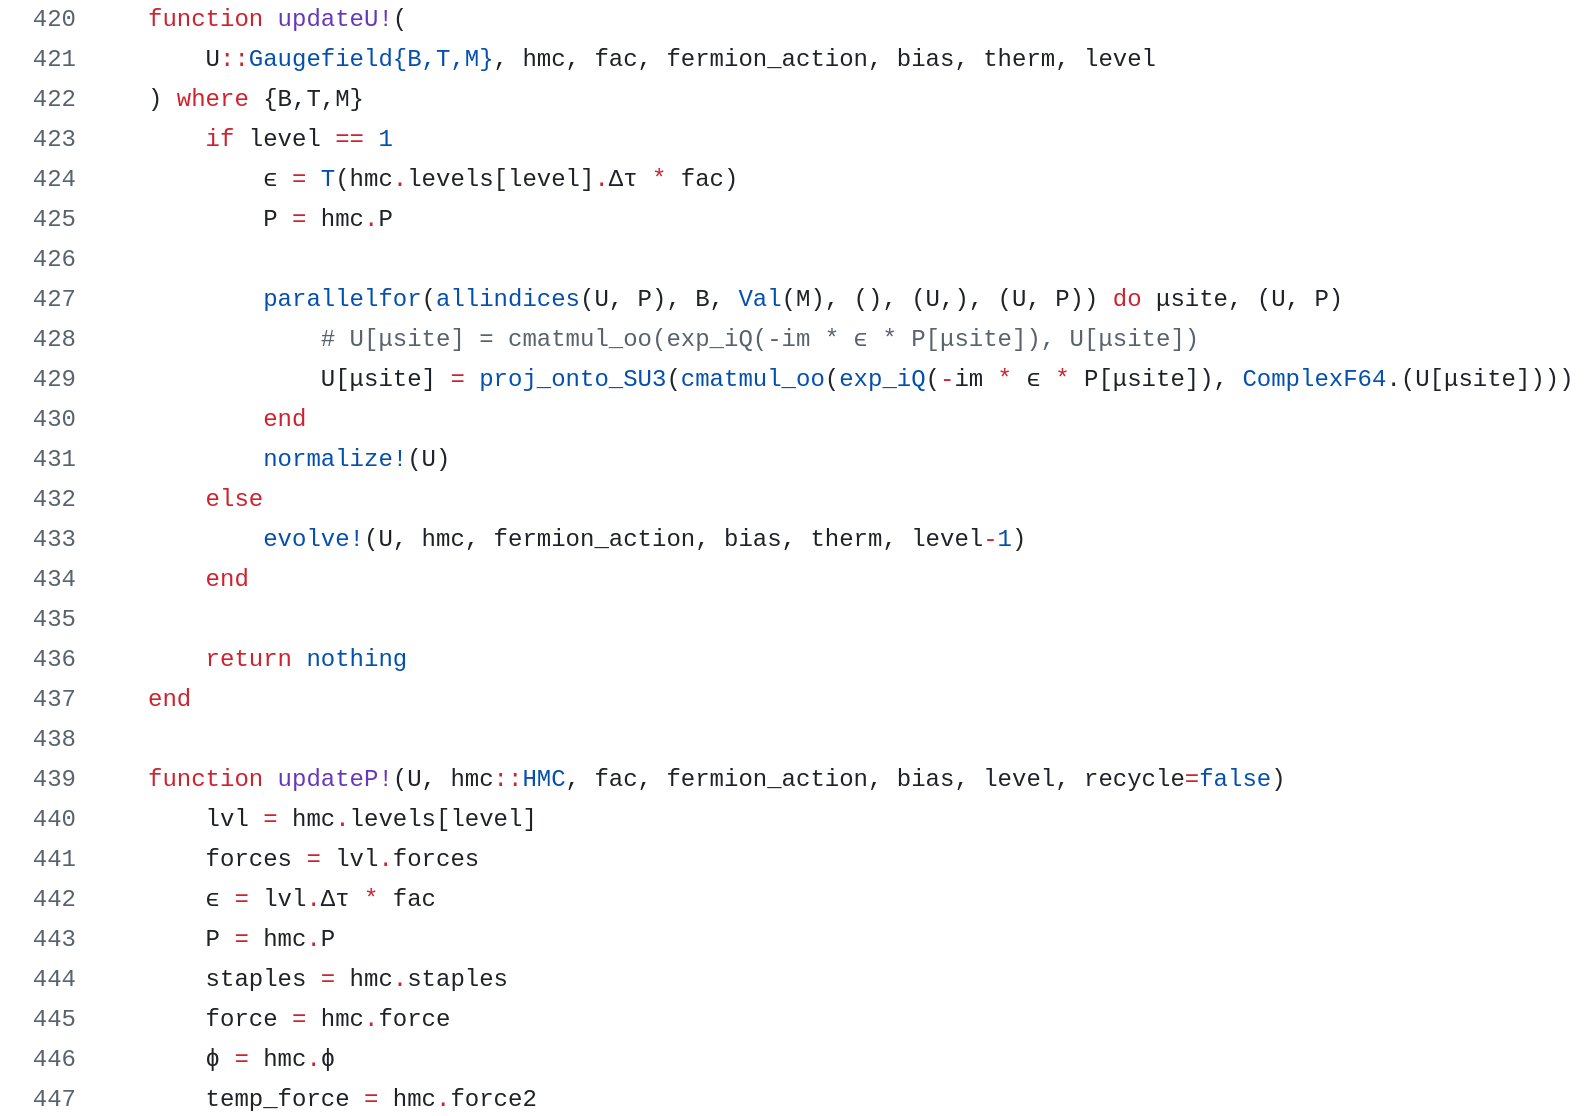
\includegraphics[width=7.29167in,height=4.16667in]{codesnippet.png}

\textbf{Veröffentlichung und Lesen von Artikeln}
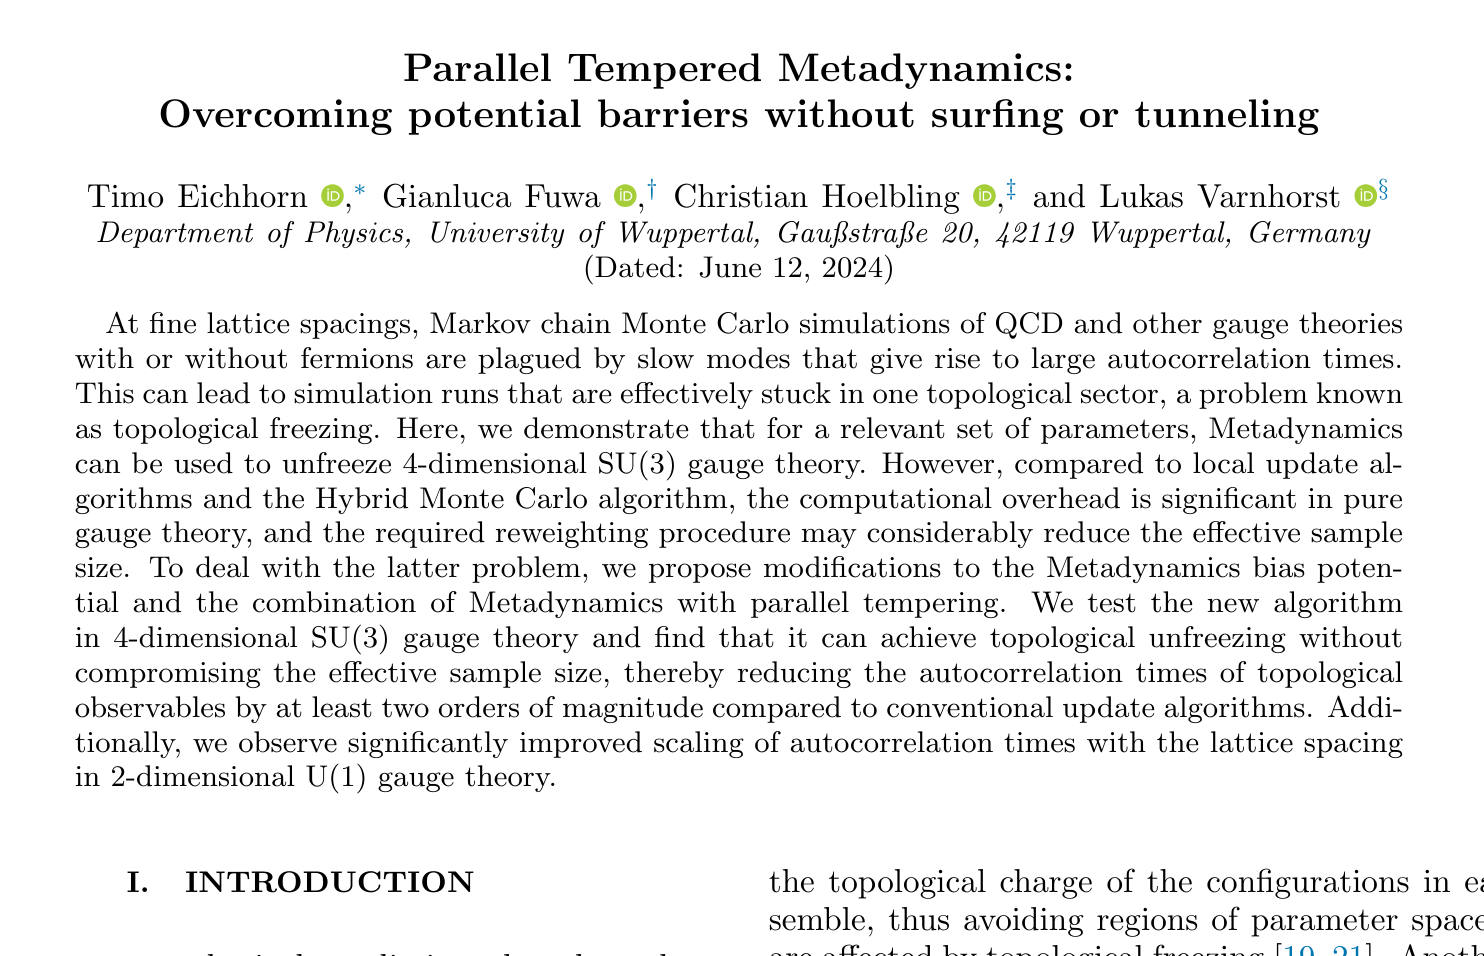
\includegraphics[width=8.33333in,height=4.6875in]{papersnippet.png}

\textbf{      Lehre      }
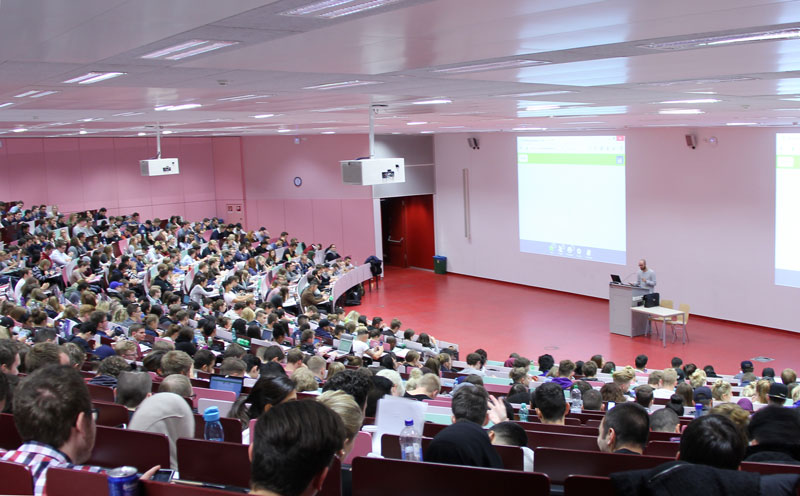
\includegraphics[width=7.29167in,height=4.16667in]{lehresnippet.jpg}

\textbf{Diskussion mit Physiker:innen weltweit auf Konferenzen oder
Workshops}
\includegraphics[width=4.6875in,height=5.72917in]{ectpicture.jpg}
\end{frame}

\begin{frame}{Warum Physik studieren?}
\phantomsection\label{warum-physik-studieren}
\begin{itemize}
\tightlist
\item
  Lernen, komplexe Probleme zu lösen
\item
  Sehr breite Berufsmöglichkeiten
\item
  Neugier als Job 😄
\end{itemize}
\end{frame}

\begin{frame}{Take-Home Message}
\phantomsection\label{take-home-message}
\begin{itemize}
\tightlist
\item
  Die Welt ist auf kleinster Skala extrem spannend
\item
  Die allermeisten Rechungen sind nicht mehr analytisch möglich
\item
  Lattice QCD verbindet Physik \& Informatik (ohne langweiligen IT Kram)
\item
  Vielleicht sitzt hier eine zukünftige Physikerin / ein zukünftiger
  Physiker 😉
\end{itemize}
\end{frame}

\begin{frame}{Fragen?}
\phantomsection\label{fragen}
\end{frame}

\section{Danke fürs Zuhören!}\label{danke-fuxfcrs-zuhuxf6ren}




\end{document}
